
\subsection{Problem 2 - Linearization}
In this section we approximate the equations of motions: (\ref{eq:pitch}), (\ref{eq:elevation}), (\ref{eq:travel}) around our desired operating point of ${p^*}={e^*}={\lambda^*}=0$


 \subsubsection{Linerizing the euqations of motions}
 
 %---------------------------------
 
 %Transform equation
 %---------------------------------
 
We transform the equations of motions in (\ref{eq:transform}) using a new coordinatte transofrmation (\ref{eq:transform}) 
\begin{equation} \label{eq:transform}
\begin{bmatrix}
    \tilde{p}\\
    \tilde{e}\\
    \tilde{\lambda}
    \end{bmatrix}
    =
    \begin{bmatrix}
        p\\
        e\\
        \lambda
    \end{bmatrix}
    -
    \begin{bmatrix}
        p^*\\
        e^*\\
        \lambda^*
    \end{bmatrix}
   \text{   and   }
    \begin{bmatrix}
         \tilde{V_s}\\
    \tilde{V_d}
    \end{bmatrix}
    =
    \begin{bmatrix}
        V_s\\
        V_d
    \end{bmatrix}
    -
    \begin{bmatrix}
     V_s^*\\
     V_d^*
    \end{bmatrix}
\end{equation} %end coordinate transofrmation

We set the derivative of our full state vector to zero, to find the equilibruim points of the system. Assuming $(\dot{p}, \dot{e},\dot{\lambda})^T=(0,0,0)^T \Rightarrow 
(\ddot{p}, \ddot{e},\ddot{\lambda})^T=(0,0,0)^T$
%-------------------------------------------------------

%               This need to be changed to include the other equatinons.

%------------------------------------------------------
\begin{align}
    J_p \ddot{p} &= L_1 V_d^* = 0 \quad &\Rightarrow \quad V_d^* &= 0  \\
    J_e \ddot{e} &= L_2 \cos(e^*) + L_3V_s^* \cos(p^*) = 0 \quad &\Rightarrow \quad V_s^* &= -\frac{L_2}{L_3} \label{eq:vs_eq} \\
   J_\lambda \ddot{\lambda}&=L_4V_s\cos({e}^*)\sin({p}^*)=0
   \end{align}


Transforming the equations of motions (\ref{eq:pitch}) - (\ref{eq:travel}) using equation (\ref{eq:transform}) we get the following:

\begin{subequations} \label{system_transformation}
\begin{align}
    J_p \ddot{p} = L_1 V_d \quad &\Rightarrow 
    \quad J_p \ddot{\tilde{p}}
    = L_1 \left( \tilde{V_d} - V_d^* \right)
    \\
    J_e \ddot{e} = L_2 \cos(e) + L_3 V_s \cos(p) \quad &\Rightarrow \quad J_e \ddot{\tilde{e}} = L_2 \cos(\tilde{e}) + L_3 \left( \tilde{V_s} + V_s^* \right) \cos(\tilde{p})
    \\
    J_\lambda \ddot{\lambda} = L_4 V_s \cos(e) \sin(p) \quad &\Rightarrow \quad J_\lambda \ddot{\tilde{\lambda}} = L_4 \left( \tilde{V_s} + V_s^* \right) \cos(\tilde{e}) \sin(\tilde{p})
\end{align}
\end{subequations}
The system of equations (\ref{system_transformation} a) - (\ref{system_transformation} c) is linearised around the point $({p}^*, {e}^*, \lambda^*)^T = (0, 0, 0)^T$ and 
$(\tilde{V_s},{V_s}^*)^T = (0, -\frac{L2}{L3})^T$:

%---------------------------------------------
%           Lineariseringsmatrise start
%--------------------------------------------

\[\left[ {\begin{array}{*{20}{c}}
{\ddot \tilde p}\\
{\ddot \tilde e}\\
{\ddot \tilde \lambda }
\end{array}} \right] = \left[ {\begin{array}{*{20}{c}}
{\frac{{\partial \ddot \tilde p}}{{\partial \tilde p}}}&{\frac{{\partial \ddot \tilde p}}{{\partial \tilde{e}}}}&{\frac{{\partial \ddot \tilde p}}{{\partial \tilde \lambda }}}\\
{\frac{{\partial \ddot \tilde e}}{{\partial \tilde p}}}&{\frac{{\partial \ddot \tilde e}}{{\partial \tilde e}}}&{\frac{{\partial \ddot \tilde e}}{{\partial \tilde \lambda }}}\\
{\frac{{\partial \ddot \tilde \lambda }}{{\partial \tilde p}}}&{\frac{{\partial \ddot \tilde \lambda }}{{\partial \tilde e}}}&{\frac{{\partial \ddot \tilde \lambda }}{{\partial \tilde \lambda }}}
\end{array}} \right]\left[ {\begin{array}{*{20}{c}}
{\tilde p}\\
{\tilde e}\\
{\tilde \lambda }
\end{array}} \right] + \left[ {\begin{array}{*{20}{c}}
{\frac{{\partial \ddot \tilde p}}{{\partial {{\tilde V}_d}}}}&{\frac{{\partial \ddot \tilde p}}{{\partial {{\tilde V}_s}}}}\\
{\frac{{\partial \ddot \tilde e}}{{\partial {{\tilde V}_d}}}}&{\frac{{\partial \ddot \tilde e}}{{\partial {{\tilde V}_s}}}}\\
{\frac{{\partial \ddot \tilde \lambda }}{{\partial {{\tilde V}_d}}}}&{\frac{{\partial \ddot \tilde \lambda }}{{\partial {{\tilde V}_s}}}}
\end{array}} \right]\left[ {\begin{array}{*{20}{c}}
{{{\tilde V}_d}}\\
{{{\tilde V}_s}}
\end{array}} \right]\]

%Lineariseringsmatrise slutt
%
%Matrise med partielderiverte start


\[\left[ {\begin{array}{*{20}{c}}
{\ddot{\tilde p}}\\
{\ddot {\tilde e}}\\
{\ddot {\tilde \lambda} }
\end{array}} \right] = \left[ {\begin{array}{*{20}{c}}
0   &0  &   0\\
{\frac{-L_3\left( \tilde{V_s} + V_s^* \right)\sin(\tilde{p})}{J_e}}   &{\frac{-L_2\sin(\tilde{e})}{J_e}}  &   0\\
{\frac{ L_4 \left( \tilde{V_s} + V_s^* \right) \cos(\tilde{e}) \cos(\tilde{p})
}{J_\lambda}}    &\frac{- L_4 \left( \tilde{V_s} + V_s^* \right) \sin(\tilde{e}) \sin(\tilde{p})
}{J_\lambda}}  &   0
\end{array}} \right]\left[ {\begin{array}{*{20}{c}}
{\tilde p}\\
{\tilde e}\\
{\tilde \lambda }
\end{array}} \right] + \left[ {\begin{array}{*{20}{c}}
\frac{L_1}{J_p}   &   0\\
0   &   \frac{L_3\cos(\tilde{p})}{J_e}\\
0   &   \frac{L_4\cos(\tilde{e})\sin(\tilde{p})}{J_\lambda}
\end{array}} \right]\left[ 
{\begin{array}{*{20}{c}}
{{{\tilde V}_d}}\\
{{{\tilde V}_s}}
\end{array}} \right]\]


{\left. {\left[ {\begin{array}{*{20}{c}}
{\ddot {\tilde p}}\\
{\ddot {\tilde e}}\\
{\ddot {\tilde \lambda }}
\end{array}} \right]} 2 = \left[ {\begin{array}{*{20}{c}}
0&0&0\\
0&0&0\\
{{K_3}}&0&0
\end{array}} \right]\left[ {\begin{array}{*{20}{c}}
{\tilde p}\\
{\tilde e}\\
{\tilde \lambda }
\end{array}} \right] + \left[ {\begin{array}{*{20}{c}}
{{K_1}}&0\\
0&{{K_2}}\\
0&0
\end{array}} \right]\left[ {\begin{array}{*{20}{c}}
{{{\tilde V}_d}}\\
{{{\tilde V}_s}}
\end{array}} \right]

Which is the same as the following equations:
\begin{subequations} \label{linearizedEquations}
\begin{align}
    \ddot{\tilde{p}} &= K_1 \tilde{V_d}\label{subeq1} \\
    \ddot{\tilde{e}} &= K_2 \tilde{V_s}\label{subeq2} \\
    \ddot{\tilde{\lambda}} &= K_3 \tilde{p}\label{eq:Travel_ddot}
\end{align}
\end{subequations}
\noindent where the constants $K_1$, $K_2$ and $K_3$ are given by
\begin{subequations}
\begin{align}
    K_1 &= \frac{L_1}{J_p}  \\
    K_2 &= \frac{L_3}{J_e} \\
    K_3 &= -\frac{L_4 L_2}{J_\lambda L_3}
\end{align}
\end{subequations}
The momement of inertia constants are given by:
\begin{subequations}
\begin{align}
    J_p &= 2 m_p l_p^2 \\
    J_e &= m_c l_c^2 + 2 m_p l_h^2 \\
    J_\lambda &= m_c l_c^2 + 2 m_p (l_h^2 l_p^2)
\end{align}
\end{subequations}

Making a script in MATLAB to calculate all of the constants is done, in order to quickly change values when changing helicopters in the lab.

\textbf{Constants MATLAB-script:}
\begin{lstlisting}
% Contains the physical constants for the helicopter
init_heli 

% Measuring V at equilibrium position:
V_s_eq = 7.23169164775339; 
V_f = V_s_eq/2;
V_b = V_s_eq/2;

K_f = -(m_c*l_c-2*m_p*l_h)*g/(l_h*V_s_eq); 

% Calculating initial conditions:
J_p = 2*m_p*l_p^2;
J_e = m_c*l_c^2 + 2*m_p*l_h^2;
J_l = m_c*l_c^2+2*m_p*((l_h^2)-(l_p^2));

% Calculating L1-L4:
L1 = K_f*l_p;
L2 = (m_c*l_c-2*m_p*l_h)*g;
L3 = l_h*K_f;
L4 = l_h*K_f;

% Calculating K-constants:
K1 = L1/J_p; 
K2 = L3/J_e;
K3 = (-L4*L2)/(J_l*L3);


    
\end{lstlisting}

\subsection{Problem 3 - Feed forward control}
The first attempt to control the helicopter was done by using feed forward control, connecting the joystick x-axis directly to the voltage difference $V_d$ and the y-axis directly to the voltage sum $V_s$.

\begin{figure}[!htb]
 \centering
    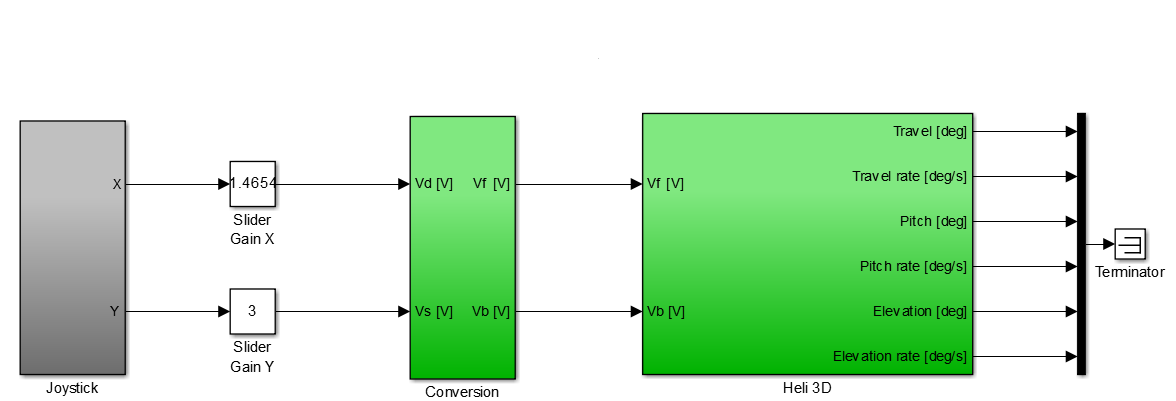
\includegraphics[scale=0.45]{images/week1_feedForward}
   
    \caption{Feed forward control with simulink}
    \label{sim:1}
\end{figure}

\subsubsection{Discussion: Physical behaviour vs. theoretical model}
In this part we will discuss some of the observations we obtained using feed forward control.

When we first attempted to control the helicopter for the first time, we began with a slider gain between the y-axis on the joystick and the voltage sum $V_s$, to find an appropriate gain to satisfy our demands on sensitivity.

Connecting the x-axis to $V_d$ would allow the joystick to interfere with the voltage difference that implies a difference in force from the two propellers. This would cause $\text{pitch angle} \neq 0$ and the helicopter starts travelling around the travel-axis. 
To make observations possible, we needed a $\text{gain} < 1$ in order to get a descent pitch sensitivity.

The theoretical model is described by the following equations from the assignment text: (\ref{eq:pitch}-\ref{eq:travel}) and the linearised version around our operation point   (\label{\label{subeq1}a) -  (\label{linearizedEquations}c)

When actually controlling the helicopter, there are some discrepancies to look into. For instance, the theoretical model does not account for external disturbances both in environment and electronics. Feeding the system with a static input does not imply a static behaviour.
The non-static behaviour makes the system more sensitive to disturbances, making it rather hard to control. Also if you approach a more dynamic kind of control, the intensity of the behaviour outperforms the human mind when it comes to time-responses on corrective inputs.

Comparing the behaviour of the system with the linearised equations, they are intended to the equilibrium point. Deviation from this point will create large differences between the theoretical linearised model and the physical behaviour.

At last, there are no feedback as long as the system is connected this way, meaning that the only feedback is what you see, and that´s rather difficult to rely on.




\subsection{Problem 4 - Estimation of $K_f$}
Before we can implement a controller that is based on the linearized equiations of motion, we need to determine the motor force constant $K_f$. By adding a "to-file" measurement on both $V_s$ and elevation angle [$e$]  in the simulink model, we were able to obtain $V_s^*$, the voltage sum at the equilibrium point.

Measurement resulted in $V_s^*=7.23V$.
\begin{align}
    {L_2} &= ({m_c}{l_c} - 2{m_p}{l_h})g \label{eq:L2} \\
       {L_3} &= {l_h}{K_f} \label{eq:L3} \\
           {V_s}^* &=-\frac{{{L_2}}}{{{L_3}}}\label{eq:Vs}
\end{align}

By using (\ref{eq:L2}), (\ref{eq:L3}) and (\ref{eq:Vs}), we calculated the motor force constant $K_f$ to be:

\begin{equation*}
    {K_f} =  - \frac{{({m_c}{l_c} - 2{m_p}{l_h})g}}{{{l_h}{V_s}^*}}
\end{equation*}
\begin{equation}\label{eq:motor force constant}
    {K_f} =  - \frac{{(1,92 \cdot 0,46 - 2 \cdot 0,72 \cdot 0,66) \cdot 9,81}}{{0,66 \cdot 7,23}}\left[ {\frac{{kg \cdot m \cdot m/{s^2}}}{{m \cdot V}}} \right]
\end{equation}

\begin{equation*}
    {K_f} = 0,1382[N/V]
\end{equation*}
\newpage

